\documentclass[12pt,a4paper]{article}
\usepackage[T1]{fontenc}
\usepackage[spanish,es-nodecimaldot]{babel}
\usepackage{tgtermes}
\usepackage{newtxmath}
\usepackage{amsmath}
\usepackage{textcomp}
\usepackage{graphicx}
\usepackage{geometry}
\usepackage{xcolor}
\usepackage{setspace}
\usepackage{titlesec}
\usepackage{tocloft}
\usepackage{fancyhdr}
\usepackage{enumitem}
\usepackage{hyperref}

\geometry{margin=2.5cm}

\definecolor{AzulPrincipal}{HTML}{0B2D4D}
\definecolor{AzulSecundario}{HTML}{1F5F8B}
\definecolor{OroAcento}{HTML}{C9A227}
\definecolor{GrisTexto}{HTML}{444444}

\hypersetup{
    colorlinks=true,
    linkcolor=black,
    urlcolor=black,
    citecolor=black,
    pdftitle={Plantilla de Informe},
    pdfauthor={Tu Nombre}
}

\setlength{\parindent}{1.25cm}
\setlength{\parskip}{0.25em}
\onehalfspacing

\setlist[itemize]{leftmargin=2.8em, labelsep=0.8em, topsep=0.35em, itemsep=0.2em}
\setlist[enumerate]{leftmargin=1.7em, topsep=0.35em, itemsep=0.2em}

\titleformat{\section}[hang]{\fontsize{18pt}{22pt}\selectfont\normalfont\color{black}}{\thesection.}{0.8em}{}
\titleformat{\subsection}[hang]{\fontsize{14pt}{17pt}\selectfont\normalfont\color{black}}{\thesubsection}{0.8em}{}

\renewcommand{\cftsecfont}{\normalfont}
\renewcommand{\cftsecpagefont}{\normalfont}
\renewcommand{\cftsubsecfont}{\normalfont}
\renewcommand{\cftsubsecpagefont}{\normalfont}
\renewcommand{\cftsecleader}{\cftdotfill{\cftdotsep}}
\renewcommand{\cftsubsecleader}{\cftdotfill{\cftdotsep}}
\renewcommand{\contentsname}{Índice}
\renewcommand{\cfttoctitlefont}{\hfill\normalfont\fontsize{18pt}{22pt}\selectfont}
\renewcommand{\cftaftertoctitle}{\hfill}

\titlespacing*{\section}{0pt}{1.1em}{0.55em}
\titlespacing*{\subsection}{0pt}{0.9em}{0.35em}

\setlength{\headheight}{30pt}

\pagestyle{fancy}
\fancyhf{}
\lhead{\small\textcolor{black!65}{\Laboratorio: \Tema}}
\rhead{}
\cfoot{\small\textcolor{black}{\thepage}}
\renewcommand{\headrulewidth}{0.4pt}
\renewcommand{\headrule}{\hbox to\headwidth{\color{black!65}\leaders\hrule height \headrulewidth\hfill}}
\renewcommand{\footrulewidth}{0pt}

\providecommand{\Universidad}{UNIVERSIDAD NACIONAL DE INGENIERÍA}
\providecommand{\Facultad}{FACULTAD DE CIENCIAS}
\providecommand{\Escuela}{ESCUELA DE FÍSICA}
\providecommand{\Curso}{CIRCUITOS ELÉCTRICOS ANALÓGICOS}
\providecommand{\Seccion}{SECCIÓN A}
\providecommand{\NumeroLaboratorio}{X}
\providecommand{\Laboratorio}{LABORATORIO N\textdegree{} \NumeroLaboratorio}
\providecommand{\Tema}{TÍTULO DE LA PRÁCTICA}
\providecommand{\RutaLogo}{logo.PNG}
\providecommand{\IntegrantesBloque}{%
\begin{enumerate}[leftmargin=1.8em,label=\arabic*.]
    \item Integrante 1 -- código
    \item Integrante 2 -- código
\end{enumerate}}
\providecommand{\FechaRealizacion}{Fecha de realización: dd de mes de aaaa - hh:mm}
\providecommand{\Ciudad}{LIMA - PERU}

\newcommand{\ConfigurarInforme}[3]{%
    \renewcommand{\NumeroLaboratorio}{#1}%
    \renewcommand{\Tema}{#2}%
    \renewcommand{\FechaRealizacion}{#3}%
}

\newcommand{\ConfigurarIntegrantes}[1]{%
    \renewcommand{\IntegrantesBloque}{#1}%
}

\providecommand{\tituloSeccion}[1]{\section{#1}}

\providecommand{\makeInformePortada}{%
\begin{titlepage}
    \thispagestyle{empty}
    \vspace*{0.65cm}
    \begin{center}
        {\Large\bfseries\color{OroAcento} \Universidad}\par
        \vspace{0.45cm}
        {\Large\bfseries\color{AzulPrincipal} \Facultad}\par
        \vspace{0.25cm}
        {\Large\bfseries\color{AzulPrincipal} \Escuela}\par
    \end{center}

    \vspace{0.1cm}
    \begin{center}
        \includegraphics[width=0.4\textwidth]{\RutaLogo}%
    \end{center}

    \vspace{0.01cm}
    \begin{center}
        {\Large\bfseries\color{AzulPrincipal} \Curso}\par
        \vspace{0.35cm}
        {\Large\bfseries\color{red} \Seccion}\par
    \end{center}

    \vspace{0.1cm}
    \begin{center}
        {\large\bfseries \Laboratorio: \Tema}\par
    \end{center}

    \vspace{0.55cm}
    \noindent{\large\textbf{INTEGRANTES DE LA MESA:} 2}\par
    \vspace{0.35cm}
    \begingroup
    \leftskip=1.15cm
    \rightskip=1.15cm
    \parindent=0pt
    \IntegrantesBloque
    \endgroup

    \vspace{0.55cm}
    \begin{center}
        {\FechaRealizacion}\par
    \end{center}

    \vfill

    \begin{center}
        {\large\bfseries \Ciudad}
    \end{center}
\end{titlepage}
}
\usepackage{tikz}
\usepackage{pgfplots}
\pgfplotsset{compat=1.18}
\renewcommand{\RutaLogo}{../../PLANTILLA/logo.PNG}
\graphicspath{{Imagenes/}}
\ConfigurarInforme{3}{PUENTE WHEATSTONE Y SENSORES RESISTIVOS}{Fecha de realización del Laboratorio N\textdegree{}3: [Completar]}

% Inicio del informe
\begin{document}
\makeInformePortada
\setcounter{page}{1}
\tableofcontents
\newpage

% Contenido del informe
\tituloSeccion{Objetivos}
\subsection{Objetivo general}
\begin{itemize}
	\item Analizar el funcionamiento del puente Wheatstone y el comportamiento de las resistencias eléctricas en sensores resistivos
\end{itemize}
\subsection{Objetivos específicos}
\begin{itemize}
    \item Configurar un puente de Wheatstone y analizar su condición de su equilibrio.
    \item Realizar mediciones de la resistencia de un termistor en función de la temperatura
	\item Medir la resistencia de una fotorresistencia bajo diferentes intensidades de la luz
\end{itemize}

\tituloSeccion{Fundamento Teórico}

\subsection{Puente Wheatstone}
El puente de Wheatstone es un circuito eléctrico formado por cuatro resistencias dispuestas en forma de puente, que se utiliza para medir una resistencia desconocida comparándola con otras resistencias conocidas. Su funcionamiento se basa en ajustar los valores de las resistencias hasta alcanzar una condición de equilibrio en la que no circula corriente por la rama central.

En la figura \ref{fig:wheatstone} se muestra el esquema del puente de Wheatstone, donde $R_1$, $R_2$, $R_3$ y $R_4$ son las resistencias del puente, $V_{in}$ es la tensión de entrada, para realizar el análisis del puente supongamos que por las mallas circulan las corrientes eléctricas $I_a. I_b \text{ e } I_c$ respectivamente.
\begin{figure}[H]
	\centering
	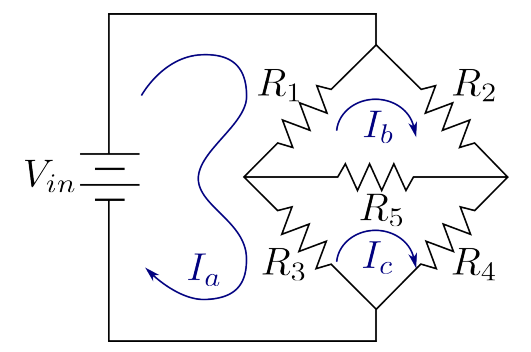
\includegraphics[width=0.5\linewidth]{Imagen1.png}
	\caption{Esquema del puente de Wheatstone.}
	\label{fig:wheatstone}
\end{figure}

De estas mallas se obtienen las siguientes ecuaciones:
\[
\left\{
\begin{aligned}
	V_{in} - R_1 (I_a - I_b) - R_3 (I_a - I_c) &= 0 \\
	-R_2 I_b - R_5 (I_b - I_c) + R_1 (I_a - I_b) &= 0 \\
	R_3 (I_c - I_a) + R_5 (I_c - I_b) + R_4 I_c &= 0
\end{aligned}
\right.
\]

Ordenando estas expresiones:
\[\left\{
\begin{aligned}
	-I_a (R_1 + R_3) + I_b R_1 + I_c R_3 &= -V_{in} \\
	I_a R_1 - I_b (R_1 + R_2 + R_5) + I_c R_5 &= 0 \\
	-I_a R_3 + I_b R_5 + I_c (R_3 + R_4 + R_5) &= 0
\end{aligned}\right.
\]

Para resolver este sistema de ecuaciones usamos determinantes:
Considerando el determinante del sistema:
\begin{equation}
	\Delta = \begin{vmatrix}
		-(R_1 + R_3) & R_1 & R_3 \\
		R_1 & -(R_1 + R_2 + R_5) & R_5 \\
		-R_3 & R_5 & (R_3 + R_4 + R_5)
	\end{vmatrix}
\end{equation}

Tenemos entonces

\begin{equation}
	I_a = \frac{\begin{vmatrix}
		-V_{in} & R_1 & R_3 \\
		0 & -(R_1 + R_2 + R_5) & R_5 \\
		0 & R_5 & (R_3 + R_4 + R_5)
	\end{vmatrix}}{\Delta}
\end{equation}

\begin{equation}
	I_b = \frac{\begin{vmatrix}
		-(R_1 + R_3) & -V_{in} & R_3 \\
		R_1 & 0 & R_5 \\
		-R_3 & 0 & (R_3 + R_4 + R_5)
	\end{vmatrix}}{\Delta}
\end{equation}

\begin{equation}
	I_c = \frac{\begin{vmatrix}
		-(R_1 + R_3) & R_1 & -V_{in} \\
		R_1 & -(R_1 + R_2 + R_5) & 0 \\
		-R_3 & R_5 & 0
	\end{vmatrix}}{\Delta}
\end{equation}

Resolviendo cada determinante:
\begin{equation}
	I_a = \frac{V_{in}\left[(R_1 + R_2 + R_5)(R_3 + R_4 + R_5) + R_5^2\right]}{\Delta}
\end{equation}
\begin{equation}
	I_b = \frac{V_{in} (R_3 R_5 + R_1 (R_3 + R_4 + R_5))}{\Delta}
\end{equation}
\begin{equation}
	I_c = \frac{V_{in} (R_3 (R_1 + R_2 + R_5) - R_1 R_5)}{\Delta}
\end{equation}

Nos interesa la intensidad de corriente eléctrica que circula por el resistor $R_5$, esta se puede obtener como $I_b - I_c$:
\begin{equation}
	I_5 = I_b - I_c = \frac{V_{in} (R_1 R_4 - R_2 R_3)}{\Delta}
\end{equation}

En esta ecuación si se cumple que 
\begin{equation}
	R_1 R_4 = R_2 R_3
	\label{eq:wheatstoneequilibrio}
\end{equation}
entonces $I_5 = 0$, es decir, no circula corriente por el resistor $R_5$. Cuando esto ocurre se dice que el puente Wheatstone se encuentra en equilibrio.  Esta condición se puede utilizar para determinar el valor de una resistencia desconocida.

\bigskip
\subsection{Influencia de la temperatura en la resistividad eléctrica de los materiales}
La resistividad eléctrica de un material es una propiedad que varía con la temperatura, en mayor o menor medida, dependiendo de la naturaleza del material. En la mayoría de los conductores, esta dependencia es aproximadamente lineal, de modo que la resistividad aumenta al incrementarse la temperatura. Este comportamiento puede describirse mediante la relación
\begin{equation}
	\rho(T) = \rho_0 [1 + \alpha (T - T_0)]
\end{equation}
donde $\rho_0$ es la resistividad medida a una temperatura de referencia $T_0$ y $\alpha$ es el coeficiente de temperatura característico del material.

Por otro lado, en los semiconductores se observa un comportamiento opuesto: la resistividad disminuye de forma exponencial cuando la temperatura aumenta. Este fenómeno se modela mediante la expresión
\begin{equation}
	\rho(T) = \rho_0 e^{\frac{E_g}{K_B T}}
\end{equation}
donde $E_g$ corresponde a la energía de la banda prohibida y $K_B$ es la constante de Boltzmann. Este tipo de comportamiento refleja cómo la conductividad en los semiconductores está fuertemente influenciada por la generación de portadores de carga a medida que la temperatura se incrementa. En la figura \ref{fig:resistividad} se muestra la gráfica de la resistividad eléctrica en función de la temperatura para un conductor y un semiconductor.
\begin{figure}[H]
	\centering
	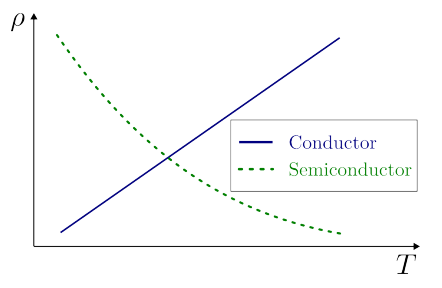
\includegraphics[width=0.5\linewidth]{Imagen2.png}
	\caption{Resistividad eléctrica en función de la temperatura para un conductor y un semiconductor.}
	\label{fig:resistividad}
\end{figure}

\subsection{Sensores}
Un sensor es un dispositivo diseñado para detectar cambios en ciertas propiedades de un material o sistema que pueden ser cuantificados. En el ámbito de los sistemas eléctricos, su función principal consiste en transformar esas variaciones en señales eléctricas, generalmente manifestadas como cambios en el voltaje, la corriente o la resistencia. Los sensores pueden clasificarse de distintas maneras: según la magnitud física que miden (como temperatura, presión, entre otras), según el tipo de señal de salida que producen (analógica o digital), o de acuerdo con el principio físico en el que se basan, como sensores resistivos, capacitivos o inductivos.

\subsubsection{Termistores}
Un termistor es un tipo de sensor resistivo cuya resistencia eléctrica cambia de manera notable en función de la temperatura. En los esquemas de circuitos, se representa mediante un símbolo específico. Existen dos categorías principales de termistores: los NTC (Negative Temperature Coefficient), cuya resistencia disminuye cuando la temperatura aumenta, y los PTC (Positive Temperature Coefficient), en los que la resistencia crece al incrementarse la temperatura. En la figura \ref{fig:termistor} se muestra el símbolo utilizado para representar un termistor en los diagramas de circuitos.
\begin{figure}[H]
	\centering
	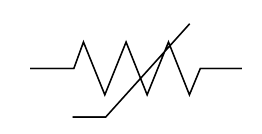
\includegraphics[width=0.3\linewidth]{Imagen3.png}
	\caption{Símbolo de un termistor en un diagrama de circuito.}
	\label{fig:termistor}
\end{figure}


\textbf{Termistores NTC:} En los termistores de tipo NTC, la resistencia eléctrica disminuye de forma considerable a medida que la temperatura aumenta. Estos dispositivos se fabrican principalmente a partir de óxidos semiconductores metálicos, como los de manganeso, níquel, cobalto o hierro. El comportamiento de la resistencia en función de la temperatura puede modelarse mediante la expresión
\begin{equation}
	R(T) = A e^{\frac{B}{T}}
\end{equation}
donde $T$ representa la temperatura, $A$ es una constante asociada a las propiedades del material y la geometría del termistor, y $B$ es una constante característica que describe su sensibilidad térmica. Este modelo refleja la fuerte dependencia no lineal entre la resistencia y la temperatura.

\textbf{Termistores PTC:} Los termistores PTC se fabrican comúnmente con titanato de bario dopado o polímeros conductores. A bajas temperaturas, la resistencia varía poco, pero a partir de una temperatura crítica $T_0$ aumenta bruscamente. En esa región se puede modelar como:
\begin{equation}
	R(T) = A e^{\frac{B}{T - T_0}}
\end{equation}
donde $A$ es una constante relacionada con el material y la geometría del termistor y $B$ representa la sensibilidad térmica. Si la temperatura sigue aumentando, la resistencia puede disminuir y afectar al dispositivo.

En la figura \ref{fig:termistores} se muestra la gráfica de la resistencia de un termistor NTC y un PTC en función de la temperatura.
\begin{figure}[H]
	\centering
	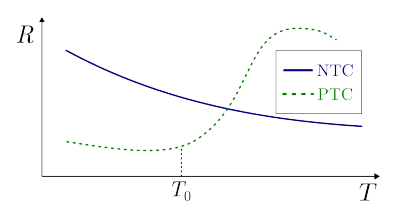
\includegraphics[width=0.5\linewidth]{Imagen4.png}
	\caption{Resistencia de un termistor NTC y PTC en función de la temperatura.}
	\label{fig:termistores}
\end{figure}

\subsubsection{Fotorresistencia:}
La fotorresistencia, también conocida como LDR (Light Dependent Resistor), es un dispositivo cuya resistencia eléctrica disminuye cuando aumenta la intensidad de luz que incide sobre su superficie. Este comportamiento se explica por la fotoconductividad, es decir, el incremento de la conductividad de un material al ser iluminado. En la figura \ref{fig:fotorresistencia-simbolo} se muestra el símbolo utilizado para representar una fotorresistencia en los diagramas de circuitos.
\begin{figure}[H]
	\centering
	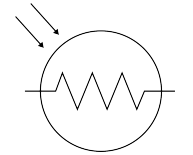
\includegraphics[width=0.3\linewidth]{Imagen5.png}
	\caption{Símbolo de una fotorresistencia en un diagrama de circuito.}
	\label{fig:fotorresistencia-simbolo}
\end{figure}
La relación entre la resistencia y la intensidad luminosa puede modelarse como:
\begin{equation}
	R(L) = AL^{-B}
\end{equation}
donde $A$ es la resistencia máxima en ausencia de luz, $L$ es la intensidad luminosa (en lux) y $B$ es una constante que depende del material y la construcción del dispositivo. En la figura \ref{fig:fotorresistencia} se muestra el comportamiento de la resistencia del LDR con la intensidad de la luz.
\begin{figure}[H]
	\centering
	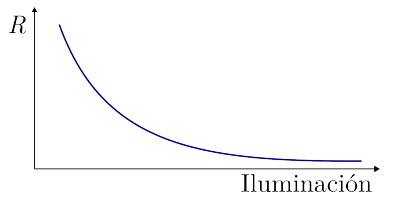
\includegraphics[width=0.5\linewidth]{Imagen6.png}
	\caption{Comportamiento de la resistencia del LDR con la intensidad de la luz.}
	\label{fig:fotorresistencia}
\end{figure}

\tituloSeccion{Materiales e indicaciones}
\begin{itemize}
    \item Fuente de voltaje DC: Fuente casera de voltaje continuo otorgado por la facultad, con salidas de voltaje predeterminadas como 1.5V, 5V y 15V, además de una perilla que regula la salida del voltaje y muestra en pantalla la cantidad exacta. Para su uso, se deben conectar los cables de salida a los terminales correspondientes del circuito, asegurándose de respetar la polaridad (positivo y negativo).
    \item Multímetro digital: Instrumento de medición, modelo PRASEK PREMIUM PR-61C, cuyos modos de operación son ohmímetro, voltímetro y amperímetro. Su número de dígitos es de 4 y presenta las siguientes escalas:
    \begin{enumerate}
        \item Resistencia: 600 $\Omega$, 6 $k\Omega$, 60 $k\Omega$, 600 $k\Omega$, 6 $M\Omega$ y 60 $M\Omega$.
        \item Voltaje: 60 mV, 600 mV, 6 V, 60 V, 600 V y 750 V.
        \item Corriente: 600 $\mu$A, 6000 $\mu$A, 60 mA, 600 mA, 6 A y 10 A.
        \item Impedancia de entrada: alrededor de 3000 $M\Omega$ en las escalas de 60 mV y 600 mV, y alrededor de 10 $M\Omega$ en las escalas de 6 V, 60 V, 600 V y 750 V.
    \end{enumerate}
	Para su uso, se deben conectar los cables de medición a los terminales correspondientes del multímetro, seleccionar la función deseada en el selector rotativo y realizar la medición en el circuito, asegurándose de respetar la polaridad y la configuración adecuada para cada tipo de medición.
    \item Protoboard: Es una placa de pruebas que permite realizar conexiones temporales sin necesidad de soldar. Para su uso, se deben insertar los componentes en las filas y columnas correspondientes, y realizar las conexiones utilizando cables de puente.
    \item Resistencias: Son componentes que limitan el flujo de corriente en un circuito. Para su uso, se deben identificar sus valores utilizando el código de colores o un multímetro, y conectarlas en el circuito según sea necesario.
    \item Potenciómetros: Son resistencias variables que permiten ajustar la resistencia manualmente. Para su uso, se deben conectar los terminales según el esquema del circuito y ajustar la perilla para obtener el valor de resistencia deseado.
	\item Termistor: Es un tipo de sensor resistivo cuya resistencia varía significativamente con la temperatura. Para su uso, se debe conectar en el circuito de acuerdo con el esquema proporcionado, y medir su resistencia mientras se somete a diferentes condiciones de temperatura para analizar su comportamiento.
	\item Fotorresistencia: Es un tipo de sensor resistivo cuya resistencia varía con la intensidad de la luz incidente. Para su uso, se debe conectar en el circuito de acuerdo con el esquema proporcionado, y medir su resistencia bajo diferentes condiciones de iluminación para analizar su comportamiento.
\end{itemize}

\newpage
\tituloSeccion{Procedimiento experimental}

\subsection{PASO 1: Implementación y balance del puente Wheatstone}
\begin{enumerate}
	\item Seleccionamos resistencias con valores cercanos a los indicadoos en la figura \ref{fig:wheatstone} para $R_1$, $R_2$ y $R_3$. Se midieron sus valores reales con el multímetro.
	\item Se armó el circuito de la figura \ref{fig:wheatstonecircuito} en el protoboard, utilizando las resistencias $R_1$, $R_2$ y $R_3$ escogidas.
	\begin{figure}[H]
		\centering
		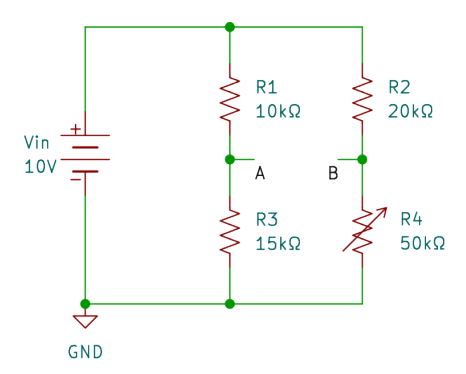
\includegraphics[width=0.5\linewidth]{Imagen7.png}
		\caption{Circuito del puente Wheatstone implementado en el protoboard.}
		\label{fig:wheatstonecircuito}
	\end{figure}
	\item De manera teórica se calculó el valor de $R_4$ usando la fórmula (\ref{eq:wheatstoneequilibrio}) para obtener la condición de equilibrio.
	\item Se escogieron diferentes valores de $R_4$ alrededor del valor teórico obtenido y se midió la diferencia de potencial en los puntos A y B en cada caso.
	\item Se registraron los valores en la tabla \ref{tab:3-1}.
\end{enumerate}

\subsection{PASO 2: Análisis del termistor}
\begin{enumerate}
	\item Utilizando un termómetro, se midió la temperatura ambiente $T_1$, con el multímetro se midió el valor de la resistencia real del termistor $R_t$ y los datos fueron registrados en la tabla \ref{tab:3-2}.
	\item Con el termómetro, se midió la temperatura de las manos de un miembro del grupo $T_2$ y luego se calentó el termistor con los dedos, de manera que las temperaturas (en la mano y en el termistor) coincidan, se midió nuevamente la resistencia del termistor, registrando los datos en la tabla \ref{tab:3-3}.
\end{enumerate}

\begin{figure}[H]
	\centering
	
\includegraphics[width=0.3\linewidth]{Imagen16.jpeg}
	\caption{Termometro registrando temperatura ambiente.}
	\label{fig:paso2-imagen16}
\end{figure}

\subsection{PASO 3: Medición con divisor de voltaje}
\begin{enumerate}
	\item Se configuró el circuito divisor con el termistor según la imagen \ref{fig:divisor} y se midió el voltaje $V_t$ en el punto de conexión entre $R_1$ y el termistor.
    \begin{figure}[H]
        \centering
		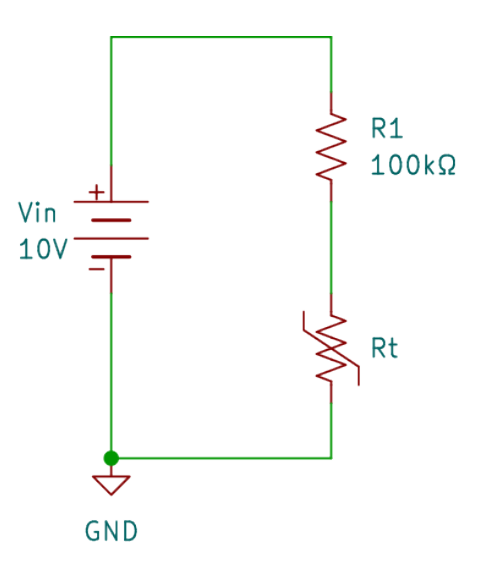
\includegraphics[width=0.4\linewidth]{Imagen8.png}
		\caption{Circuito divisor de voltaje con termistor.}
		\label{fig:divisor}
	\end{figure}
	\item Se midió el voltaje en el termistor a las temperaturas $T_1$ y $T_2$ para $R_1 = 100$ k$\Omega$ y luego para $R_1 = 50$ k$\Omega$ (valores teóricos).
	\item Se registraron los datos en las tablas \ref{tab:3-4}, \ref{tab:3-5}, \ref{tab:3-6} y \ref{tab:3-7}.
\end{enumerate}

\newpage
\subsection{PASO 4: Puente Wheatstone con termistor}
\begin{enumerate}
	\item Se armó el circuito de la figura \ref{fig:wheatstonetermistor} con el termistor en lugar de $R_2$.
	\begin{figure}[H]
		\centering
		\begin{minipage}{0.5\linewidth}
			\centering
			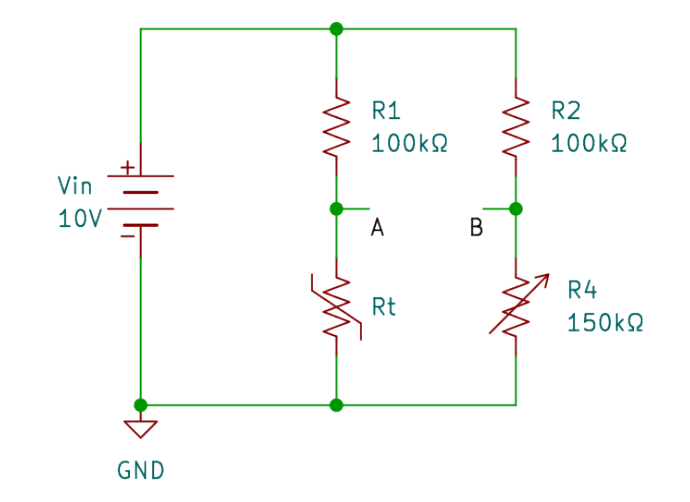
\includegraphics[width=\linewidth]{Imagen9.png}
		\end{minipage}
\hspace{0.02\linewidth}
		\begin{minipage}{0.3\linewidth}
			\centering
			
\includegraphics[width=\linewidth]{Imagen17.jpeg}
		\end{minipage}
		\caption{Circuito del puente Wheatstone con termistor.}
		\label{fig:wheatstonetermistor}
	\end{figure}
	\item A la temperatura $T_1$ se buscó el balance del puente modificando la resistencia $R_4$ y usando la ecuación (\ref{eq:wheatstoneequilibrio}) se calculó el valor de $R_t$. Los datos fueron registrados en la tabla \ref{tab:3-8}.
	\item Se repitió el procedimiento anterior pero para la temperatura $T_2$, registrando los datos en la tabla \ref{tab:3-9}.
\end{enumerate}

\subsection{PASO 5: Análisis de la fotorresistencia}
\begin{enumerate}
	\item Se midió la resistencia de la fotorresistencia con luz ambiente y con poca luz (se cubrió con un dedo).
	\item Se registraron los datos en la tabla \ref{tab:3-10}.
\end{enumerate}

\subsection{PASO 6: Divisor de voltaje con fotorresistencia}
\begin{enumerate}
	\item Se armó el divisor de voltaje con la fotorresistencia mostrado en la figura \ref{fig:divisorfotorresistencia}.
	\begin{figure}[H]
		\centering
		\begin{minipage}{0.35\linewidth}
			\centering
			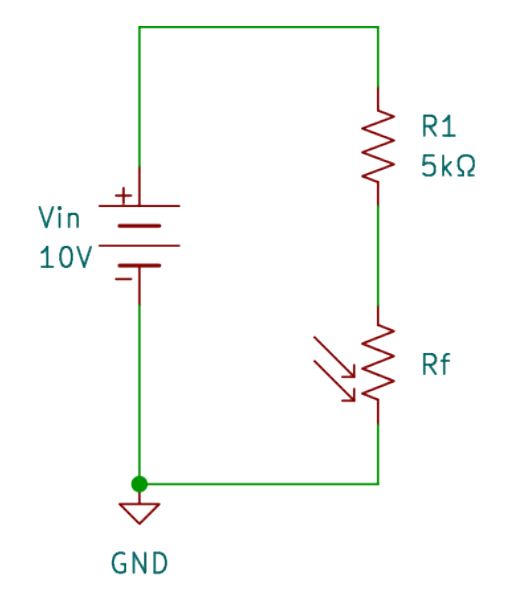
\includegraphics[width=\linewidth]{Imagen10.png}
		\end{minipage}
    \hspace{0.02\linewidth}
		\begin{minipage}{0.28\linewidth}
			\centering
			
\includegraphics[width=\linewidth]{Imagen18.jpeg}
		\end{minipage}
		\caption{Circuito divisor de voltaje con fotorresistencia.}
		\label{fig:divisorfotorresistencia}
	\end{figure}
	\item Usando la iluminación del laboratorio y cubriendo la fotorresistencia se midió el voltaje de la fotorresistencia.
	\item Usando el divisor de voltaje, calculamos la resistencia en la fotorresistencia.
	\item Se anotaron los datos en las tablas \ref{tab:3-11}, \ref{tab:3-12}, \ref{tab:3-13} y \ref{tab:3-14}.
\end{enumerate}
\bigskip

\subsection{PASO 7: Puente Wheatstone con fotorresistencia}
\begin{enumerate}
	\item Se armó el puente de Wheatstone con la fotorresistencia, según la imagen \ref{fig:wheatstonefotorresistencia}.
	\begin{figure}[H]
		\centering
		\begin{minipage}{0.5\linewidth}
			\centering
			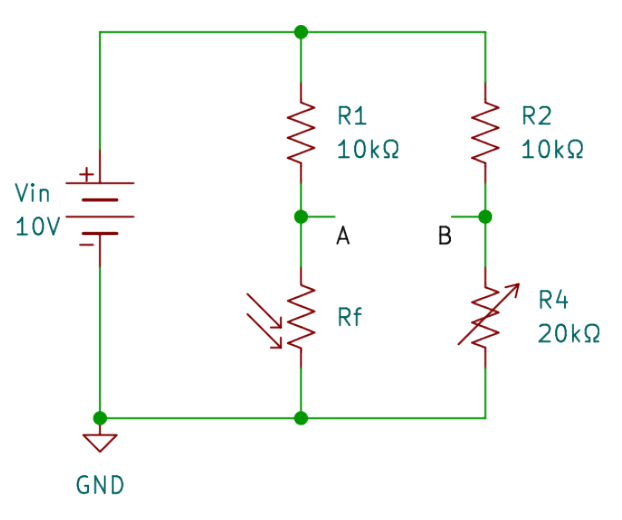
\includegraphics[width=\linewidth]{Imagen11.png}
		\end{minipage}
    \hspace{0.02\linewidth}
		\begin{minipage}{0.3\linewidth}
			\centering
			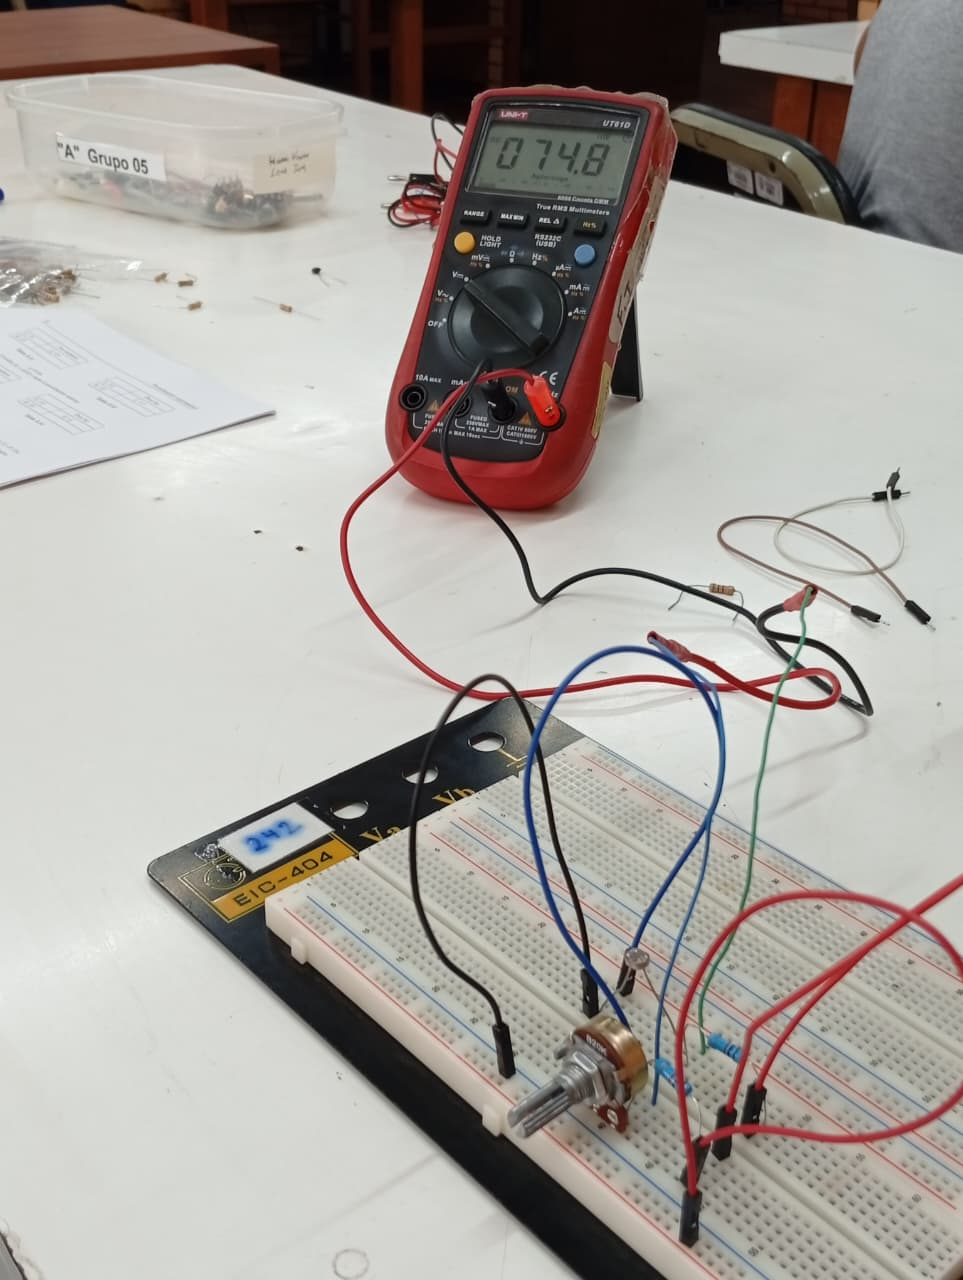
\includegraphics[width=\linewidth]{Imagen19.jpeg}
		\end{minipage}
		\caption{Circuito del puente Wheatstone con fotorresistencia.}
		\label{fig:wheatstonefotorresistencia}
	\end{figure}
	\item Con la luz del laboratorio, se buscó el balance del puente modificando la resistencia $R_4$ y usando la ecuación (\ref{eq:wheatstoneequilibrio}) se calculó el valor de $R_f$. Se registraron los datos en la tabla \ref{tab:3-15}.
	\item Se repitió el procedimiento para poca luz, registrando los datos en la tabla \ref{tab:3-16}.
\end{enumerate}
\bigskip

\tituloSeccion{Análisis de datos}

\subsection{PASO 1: Datos del puente Wheatstone}

Datos reales: 
\begin{itemize}
	\item $V_{in} = 9,9$ V
	\item $R_1 = 9,98$ k$\Omega, \quad R_2 = 19,83$ k$\Omega, \quad R_3 = 17,52$ k$\Omega$
	\item Resistor de $100$ k$\Omega$ utilizado para $R_4$.
	\item Valor teórico de $R_4$ para equilibrio: $34,81$ k$\Omega$.
\end{itemize}

\begin{table}[H]
\centering
\fontsize{9.5pt}{11.5pt}\selectfont
\renewcommand{\arraystretch}{1.2}
\setlength{\tabcolsep}{4pt}
\begin{tabular}{|C{2.1cm}|C{1.1cm}|C{1.1cm}|C{1.1cm}|C{1.1cm}|C{1.1cm}|C{1.1cm}|C{1.1cm}|C{1.1cm}|C{1.1cm}|}
\hline
\textbf{$R_4$ (k$\Omega$)} & 30,55 & 31,63 & 32,26 & 33,16 & 34,09 & 34,82 & 35,35 & 36,36 & 37,71 \\
\hline
\textbf{$V_{AB}$ (V)} & 0,31 & 0,23 & 0,18 & 0,11 & 0,05 & 0,02 & 0,03 & 0,10 & 0,19 \\
\hline
\end{tabular}
\caption{Medición de $V_{AB}$ para distintos valores de $R_4$.}
\label{tab:3-1}
\end{table}
\newpage
\textbf{ANÁLISIS:} En la tabla \ref{tab:3-1} se observa que a medida que $R_4$ se acerca al valor teórico de equilibrio (34,81 k$\Omega$), el voltaje $V_{AB}$ disminuye, alcanzando un mínimo de 0,02 V en ese punto. Esto indica que el puente está cerca del equilibrio, aunque no se logra un valor exactamente nulo debido a las tolerancias de los componentes y las mediciones. Para valores de $R_4$ menores o mayores al valor teórico, el voltaje $V_{AB}$ aumenta, lo que confirma la relación establecida por la ecuación (\ref{eq:wheatstoneequilibrio}).

\bigskip
\subsection{PASO 2: Mediciones del termistor}

\begin{table}[H]
\centering
\begin{tabular}{|C{3cm}|C{3cm}|}
\hline
\textbf{$T_1$ ($^\circ$C)} & 27,0 \\
\hline
\textbf{$R_t$ ($\Omega$)} & 8,77 k$\Omega$ \\
\hline
\end{tabular}
\caption{Medición directa del termistor a temperatura ambiente.}
\label{tab:3-2}
\end{table}

\begin{table}[H]
\centering
\begin{tabular}{|C{3cm}|C{3cm}|}
\hline
\textbf{$T_2$ ($^\circ$C)} & 35,1 \\
\hline
\textbf{$R_t$ ($\Omega$)} & 6,06 k$\Omega$ \\
\hline
\end{tabular}
\caption{Medición directa del termistor con aumento de temperatura.}
\label{tab:3-3}
\end{table}

\textbf{ANÁLISIS:} En las tablas \ref{tab:3-2} y \ref{tab:3-3} se observa que al aumentar la temperatura de 27,0 $^\circ$C a 35,1 $^\circ$C, la resistencia del termistor disminuye de 8,77 k$\Omega$ a 6,06 k$\Omega$. Este comportamiento es característico de un termistor NTC, donde la resistencia disminuye a medida que la temperatura aumenta.

\subsection{PASO 3: Divisor de voltaje con termistor}

Datos reales:
\begin{itemize}
	\item $V_{in} = 9,8$ V
	\item $R_1$: 97,8 k$\Omega$ para la primera parte y 49,17 k$\Omega$ para la segunda parte.
\end{itemize}
\begin{table}[H]
\centering
\begin{tabular}{|C{3cm}|C{3cm}|}
\hline
\textbf{$T_1$ ($^\circ$C)} & 27,0 \\
\hline
\textbf{$V_t$ (V)} & 0,81 \\
\hline
\textbf{$R_t$ ($\Omega$)} & 8,81 k$\Omega$ \\
\hline
\end{tabular}
\caption{Cálculo de $R_t$ con $R_1 = 97,8$ k$\Omega$ a $T_1$.}
\label{tab:3-4}
\end{table}

\begin{table}[H]
\centering
\begin{tabular}{|C{3cm}|C{3cm}|}
\hline
\textbf{$T_2$ ($^\circ$C)} & 35,1 \\
\hline
\textbf{$V_t$ (V)} & 0,61 \\
\hline
\textbf{$R_t$ ($\Omega$)} & 6,49 k$\Omega$ \\
\hline
\end{tabular}
\caption{Cálculo de $R_t$ con $R_1 = 97,8$ k$\Omega$ a $T_2$.}
\label{tab:3-5}
\end{table}

\begin{table}[H]
\centering
\begin{tabular}{|C{3cm}|C{3cm}|}
\hline
\textbf{$T_1$ ($^\circ$C)} & 27,0 \\
\hline
\textbf{$V_t$ (V)} & 1,50 \\
\hline
\textbf{$R_t$ ($\Omega$)} & 8,89 k$\Omega$ \\
\hline
\end{tabular}
\caption{Cálculo de $R_t$ con $R_1 = 49,17$ k$\Omega$ a $T_1$.}
\label{tab:3-6}
\end{table}

\begin{table}[H]
\centering
\begin{tabular}{|C{3cm}|C{3cm}|}
\hline
\textbf{$T_2$ ($^\circ$C)} & 35,1 \\
\hline
\textbf{$V_t$ (V)} & 1,11 \\
\hline
\textbf{$R_t$ ($\Omega$)} & 6,28 k$\Omega$ \\
\hline
\end{tabular}
\caption{Cálculo de $R_t$ con $R_1 = 49,17$ k$\Omega$ a $T_2$.}
\label{tab:3-7}
\end{table}

\textbf{ANÁLISIS:} En las tablas \ref{tab:3-4} a \ref{tab:3-7} se observa que los valores de $R_t$ calculados a partir del divisor de voltaje son cercanos a los valores medidos directamente con el multímetro en el paso anterior. Sin embargo, hay pequeñas discrepancias que pueden atribuirse a las tolerancias de los componentes, las mediciones y la precisión del multímetro. A pesar de estas diferencias, el comportamiento general del termistor sigue siendo consistente con un dispositivo NTC, mostrando una disminución en la resistencia al aumentar la temperatura.
\bigskip

\subsection{PASO 4: Puente Wheatstone con termistor}

Datos reales:
\begin{itemize}
	\item $V_{in} = 9,8$ V
	\item $R_1 = 97,8$ k$\Omega, \quad R_2 = 97,7$ k$\Omega$
	\item Potenciometro de 20 k$\Omega$ utilizado para $R_4$
\end{itemize}
\begin{table}[H]
\centering
\begin{tabular}{|C{3cm}|C{3cm}|}
\hline
\textbf{$T_1$ ($^\circ$C)} & 27,0 \\
\hline
\textbf{$R_4$ ($\Omega$)} & 8,80 k$\Omega$ \\
\hline
\textbf{$R_t$ ($\Omega$)} & 8,77 k$\Omega$ \\
\hline
\end{tabular}
\caption{Balance del puente con termistor a $T_1$.}
\label{tab:3-8}
\end{table}

\begin{table}[H]
\centering
\begin{tabular}{|C{3cm}|C{3cm}|}
\hline
\textbf{$T_2$ ($^\circ$C)} & 35,1 \\
\hline
\textbf{$R_4$ ($\Omega$)} & 6,01 k$\Omega$ \\
\hline
\textbf{$R_t$ ($\Omega$)} & 6,06 k$\Omega$ \\
\hline
\end{tabular}
\caption{Balance del puente con termistor a $T_2$.}
\label{tab:3-9}
\end{table}

\textbf{ANÁLISIS:} En las tablas \ref{tab:3-8} y \ref{tab:3-9} se observa que al ajustar la resistencia $R_4$ para balancear el puente, los valores de $R_t$ calculados a partir de la condición de equilibrio son muy cercanos a los valores medidos directamente con el multímetro en el paso 2. Esto indica que el puente Wheatstone es una herramienta efectiva para determinar la resistencia del termistor bajo diferentes condiciones de temperatura, y que el comportamiento del termistor sigue siendo consistente con un dispositivo NTC.
\bigskip

\subsection{PASO 5: Mediciones de fotorresistencia}

\begin{table}[H]
\centering
\begin{tabular}{|C{3.2cm}|C{3.2cm}|C{3.2cm}|}
\hline
\textbf{} & {Luz ambiente} & \textbf{Poca luz} \\
\hline
$R_f (\Omega)$ & 1,57 k$\Omega$ & 6,25 k$\Omega$ \\
\hline
\end{tabular}
\caption{Medición directa de $R_f$ con multímetro.}
\label{tab:3-10}
\end{table}

\textbf{ANÁLISIS:} En la tabla \ref{tab:3-10} se observa que la resistencia de la fotorresistencia es significativamente menor en condiciones de luz ambiente (1,57 k$\Omega$) en comparación con condiciones de poca luz (6,25 k$\Omega$). Este comportamiento es característico de una fotorresistencia, donde la resistencia disminuye al aumentar la intensidad de la luz incidente.
\bigskip

\subsection{PASO 6: Divisor de voltaje con fotorresistencia}

Datos reales:
\begin{itemize}
	\item $V_{in} = 9,9$ V
	\item $R_1$: 4,88 k$\Omega$ para la primera parte y 9,97 k$\Omega$ para la segunda parte.
\end{itemize}

\begin{table}[H]
\centering
\begin{tabular}{|C{3cm}|C{3cm}|}
\hline
	& \textbf{Luz ambiente} \\
\hline
\textbf{$V_f$ (V)} & 2,40 \\
\hline
\textbf{$R_f$ ($\Omega$)} & 1,56 k$\Omega$ \\
\hline
\end{tabular}
\caption{Luz ambiente con $R_1 = 4,88$ k$\Omega$.}
\label{tab:3-11}
\end{table}

\begin{table}[H]
\centering
\begin{tabular}{|C{3cm}|C{3cm}|}
\hline
	& \textbf{Poca luz} \\
\hline
\textbf{$V_f$ (V)} & 5,75 \\
\hline
\textbf{$R_f$ ($\Omega$)} & 6,76 k$\Omega$ \\
\hline
\end{tabular}
\caption{Poca luz con $R_1 = 9,97$ k$\Omega$.}
\label{tab:3-12}
\end{table}

\begin{table}[H]
\centering
\begin{tabular}{|C{3cm}|C{3cm}|}
\hline
	& \textbf{Luz ambiente} \\
\hline
\textbf{$V_f$ (V)} & 1,22 \\
\hline
\textbf{$R_f$ ($\Omega$)} & 1,40 k$\Omega$ \\
\hline
\end{tabular}
\caption{Luz ambiente con $R_1 = 4,88$ k$\Omega$.}
\label{tab:3-13}
\end{table}

\begin{table}[H]
\centering
\begin{tabular}{|C{3cm}|C{3cm}|}
\hline
	& \textbf{Poca luz} \\
\hline
\textbf{$V_f$ (V)} & 4,16 \\
\hline
\textbf{$R_f$ ($\Omega$)} & 7,23 k$\Omega$ \\
\hline
\end{tabular}
\caption{Poca luz con $R_1 = 9,97$ k$\Omega$.}
\label{tab:3-14}
\end{table}

\textbf{ANÁLISIS:} En las tablas \ref{tab:3-11} a \ref{tab:3-14} se observa que los valores de $R_f$ calculados a partir del divisor de voltaje son cercanos a los valores medidos directamente con el multímetro en el paso 5. Sin embargo, hay pequeñas discrepancias que pueden atribuirse a las tolerancias de los componentes, las mediciones y la precisión del multímetro. A pesar de estas diferencias, el comportamiento general de la fotorresistencia sigue siendo consistente con un dispositivo LDR, mostrando una disminución en la resistencia al aumentar la intensidad de la luz incidente.
\bigskip

\subsection{PASO 7: Puente Wheatstone con fotorresistencia}

Valores reales:
\begin{itemize}
	\item $V_{in} = 9,8$ V
	\item $R_1 = 9,98$ k$\Omega, \quad R_2 = 10$ k$\Omega$
	\item Potenciometro de 20 k$\Omega$ utilizado para $R_4$
\end{itemize}

\begin{table}[H]
\centering
\begin{tabular}{|C{3cm}|C{3cm}|C{3cm}|}
\hline
	& \textbf{Luz ambiente} \\
\hline
\textbf{$R_4$ ($\Omega$)} & 1,59 k$\Omega$ \\
\hline
\textbf{$R_f$ ($\Omega$)} & 1,586 k$\Omega$ \\
\hline
\end{tabular}
\caption{Balance del puente en luz ambiente.}
\label{tab:3-15}
\end{table}

\begin{table}[H]
\centering
\begin{tabular}{|C{3cm}|C{3cm}|}
\hline
	& \textbf{Poca luz} \\
\hline
\textbf{$R_4$ ($\Omega$)} & 6,18 k$\Omega$ \\
\hline
\textbf{$R_f$ ($\Omega$)} & 6,167 k$\Omega$ \\
\hline
\end{tabular}
\caption{Balance del puente en condición de poca luz.}
\label{tab:3-16}
\end{table}

\textbf{ANÁLISIS:} En las tablas \ref{tab:3-15} y \ref{tab:3-16} se observa que al ajustar la resistencia $R_4$ para balancear el puente, los valores de $R_f$ calculados a partir de la condición de equilibrio son muy cercanos a los valores medidos directamente con el multímetro en el paso 5. Esto indica que el puente Wheatstone es una herramienta efectiva para determinar la resistencia de la fotorresistencia bajo diferentes condiciones de iluminación, y que el comportamiento del LDR sigue siendo consistente con un dispositivo cuya resistencia disminuye al aumentar la intensidad de la luz incidente.
\bigskip

\newpage
\tituloSeccion{Discusión de resultados}

En el PASO 1 (tabla \ref{tab:3-1}), el voltaje mínimo $V_{AB} = 0,02$ V se alcanzó en $R_4 = 34,82$ k$\Omega$, muy próximo al valor teórico de 34,81 k$\Omega$, validando la condición de equilibrio del puente ($R_1 R_4 = R_2 R_3$). La pequeña discrepancia (0,01 k$\Omega$, equivalente a 0,03\%) refleja las tolerancias inherentes de los componentes de laboratorio. 

En los PASOS 2 a 4 con el termistor, la resistencia disminuyó de 8,77 k$\Omega$ a 27,0 °C a 6,06 k$\Omega$ a 35,1 °C (tablas \ref{tab:3-2} y \ref{tab:3-3}), confirmando comportamiento NTC. Los valores calculados mediante divisor de voltaje (tablas \ref{tab:3-4} a \ref{tab:3-7}) difieren menos del 2\% de las mediciones directas, y el balance del puente (tablas \ref{tab:3-8} y \ref{tab:3-9}) mostró diferencias menores al 0,5\% entre $R_4$ calculado y $R_t$ medido, indicando concordancia entre los tres métodos.

En los PASOS 5 a 7 con la fotorresistencia, la resistencia fue 1,57 k$\Omega$ en luz ambiente y 6,25 k$\Omega$ en poca luz (tabla \ref{tab:3-10}), validando comportamiento LDR. Los cálculos del divisor de voltaje (tablas \ref{tab:3-11} a \ref{tab:3-14}) y el balance del puente (tablas \ref{tab:3-15} y \ref{tab:3-16}) mantuvieron concordancia similar. Estas discrepancias menores son atribuibles a las tolerancias estándar de resistencias (5\%) y la precisión del multímetro, siendo aceptables para aplicaciones prácticas.

\tituloSeccion{Actividades adicionales}
\begin{enumerate}
\item \textit{A partir de los datos del PASO 1, haga un gráfico teórico y experimental de $V_{AB}/V_{in}$ vs. $R_4$ y determine aproximadamente el valor de $R_4$ para el cual el puente está balanceado.}

\begin{figure}[H]
\centering
\begin{tikzpicture}
\begin{axis}[
	width=0.95\linewidth,
	height=8cm,
	xlabel={$R_4$ (k$\Omega$)},
	ylabel={$|V_{AB}/V_{in}|$ ($\times 10^{-2}$)},
	xmin=30.3, xmax=37.9,
	ymin=0, ymax=3.5,
	axis lines=left,
	grid=major,
	minor tick num=1,
	minor grid style={gray!25},
	major grid style={gray!50},
	tick align=outside,
	line width=0.8pt,
	xtick={30.5,31.5,32.5,33.5,34.5,35.5,36.5,37.5},
	ytick={0,0.5,1.0,1.5,2.0,2.5,3.0,3.5},
	xlabel style={font=\scriptsize},
	ylabel style={font=\scriptsize},
	xticklabel style={font=\scriptsize},
	yticklabel style={font=\scriptsize,/pgf/number format/fixed,/pgf/number format/precision=1},
	legend style={at={(0.98,0.98)},anchor=north east,draw=none,fill=white,font=\small},
	clip=false,
]
\addplot[very thick, blue!80!black, domain=30.5:37.7, samples=300] {100*abs(17.52/(9.98+17.52) - x/(19.83+x))};
\addlegendentry{Modelo teórico}

\addplot[thick, red!85!black, mark=*, mark size=2.2pt] coordinates {
	(30.55,3.13)
	(31.63,2.32)
	(32.26,1.82)
	(33.16,1.11)
	(34.01,0.51)
	(34.82,0.20)
	(35.35,0.30)
	(36.36,1.01)
	(37.71,1.92)
};
\addlegendentry{Datos experimentales}

\addplot[dashed, thick, gray!75] coordinates {(34.81,0) (34.81,3.5)};

\addplot[densely dotted, thick, gray!70] coordinates {(30.3,0) (37.9,0)};

\node[anchor=center, font=\scriptsize, fill=white, inner sep=1.5pt, draw=none] at (axis cs:34.9,1.35) {$R_4=34.82$ k$\Omega$, $V_{AB}/V_{in}\approx 0.20\times 10^{-2}$};
\end{axis}
\end{tikzpicture}
\caption{Gráfica teórica y experimental de $V_{AB}/V_{in}$ frente a $R_4$ en el PASO 1.}
\label{fig:grafica-paso1}
\end{figure}

De la gráfica se observa que el puente se balancea aproximadamente en $R_4 \approx 34,81$ k$\Omega$, valor en el que la curva teórica y los datos experimentales se acercan al mínimo de $V_{AB}/V_{in}$.
\newpage
\item \textit{A partir de los experimentos realizados con el termistor, deduzca que tipo de termistor es.}
\smallskip

El termistor es de tipo NTC, porque en los PASOS 2, 3 y 4 su resistencia disminuye cuando aumenta la temperatura. Ese comportamiento se repite tanto en la medición directa como en el divisor de voltaje y en el puente Wheatstone.

\item \textit{A partir de los experimentos realizados con la fotorresistencia comente su comportamiento.}
\smallskip

La fotorresistencia se comporta como una LDR: su resistencia es menor con luz ambiente y aumenta cuando se cubre o disminuye la iluminación. Esto se verifica en los PASOS 5, 6 y 7, donde los valores medidos cambian de forma consistente con la intensidad de luz.
\end{enumerate}

\tituloSeccion{Conclusiones}

\begin{itemize}
	\item El puente Wheatstone demostró ser preciso para medir resistencias desconocidas mediante comparación relativa. El error de balance fue de apenas 0,03\% (PASO 1), validando la ecuación de equilibrio $R_1 R_4 = R_2 R_3$.
	\item El termistor utilizado es de tipo NTC. La resistencia pasó de 8,77 k$\Omega$ a 27,0 °C a 6,06 k$\Omega$ a 35,1 °C (PASOS 2-4), correspondiéndole una sensibilidad de aproximadamente $-3,81$ k$\Omega$/°C en ese rango de temperatura.
	\item La fotorresistencia exhibió comportamiento LDR consistente (PASOS 5-7). Su resistencia varió desde 1,57 k$\Omega$ en luz ambiente a 6,25 k$\Omega$ en poca luz, demostrando alta sensibilidad a cambios de iluminación.
	\item Los valores de resistencia calculados mediante los tres métodos (multímetro directo, divisor de voltaje y puente Wheatstone) coincidieron dentro de tolerancias menores al 2\%, confirmando la validez teórica y práctica de las técnicas empleadas.
\end{itemize}

\tituloSeccion{Bibliografía}
    \begin{itemize}
        \item JAMES J. BROPHY, \textit{Basic electronics for scientists}, $5^{Th}$ Edition, McGraw Hill.
        \item UNI-FC, \textit{Circuitos Electrónicos Analógicos: Guía de laboratorio del experimento 3}, 2026
    \end{itemize}

\tituloSeccion{Anexos}

\begin{figure}[H]
    \centering
    \begin{minipage}{0.48\linewidth}
        \centering
        
\includegraphics[width=\linewidth]{Imagen12.jpeg}
        \caption{Anexo 1: PASO1, PASO 2 y PASO 3.}
        \label{anexo1}
    \end{minipage}
    \hspace{0.02\linewidth}
    \begin{minipage}{0.48\linewidth}
        \centering
        
\includegraphics[width=\linewidth]{Imagen13.jpeg}
        \caption{Anexo 2: PASO 3 Y PASO 4.}
        \label{anexo2}
    \end{minipage}
\end{figure}

\begin{figure}[H]
    \centering
    \begin{minipage}{0.48\linewidth}
        \centering
        
\includegraphics[width=\linewidth]{Imagen14.jpeg}
        \caption{Anexo 3: PASO 5 Y PASO 6.}
        \label{anexo3}
    \end{minipage}
    \hspace{0.02\linewidth}
    \begin{minipage}{0.48\linewidth}
        \centering
        
\includegraphics[width=\linewidth]{Imagen15.jpeg}
        \caption{Anexo 4: PASO 6 Y PASO 7.}
        \label{anexo4}
    \end{minipage}
\end{figure}

\end{document}
